
\chapter{Problèmes introductifs}

	\initial{P}{our} mettre le lecteur en appétit, nous mettons à disposition quelques problèmes dont la résolution nécessite les outils mathématiques que nous allons aborder. Nous invitons le lecteur à se creuser la tête avant même de lire les débuts de résolution que nous avons mis à disposition, au moins quelques minutes avec un papier et un crayon. Le lecteur peut revenir à ces problèmes à sa guise, même si nous l'y invitons lorsque les outils nécessaires ont été abordés.

	\paragraph{Problème A} Soit un segment $[AB]$ de mesure 1 (peu importe l'unité). Soit $M$ un point mobile sur $[AB]$. On construit le carré de côté $[AM]$ et le triangle équilatéral de côté $[BM]$.
	Trouver la position du point $M$ tel que le périmètre du carré égale le périmètre du triangle équilatéral.

	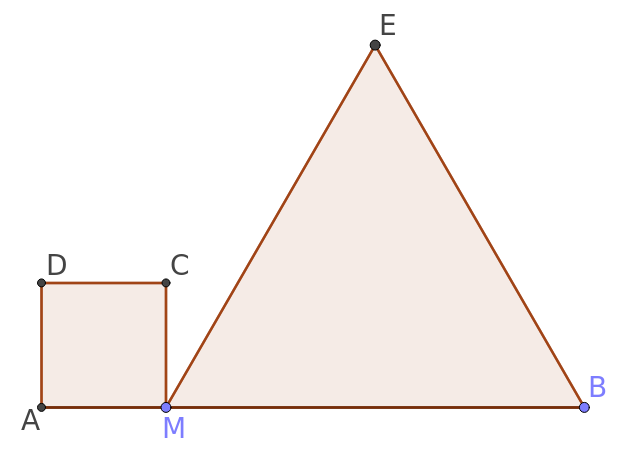
\includegraphics[width=0.3\textwidth]{image/calcul/pbtricar1.png}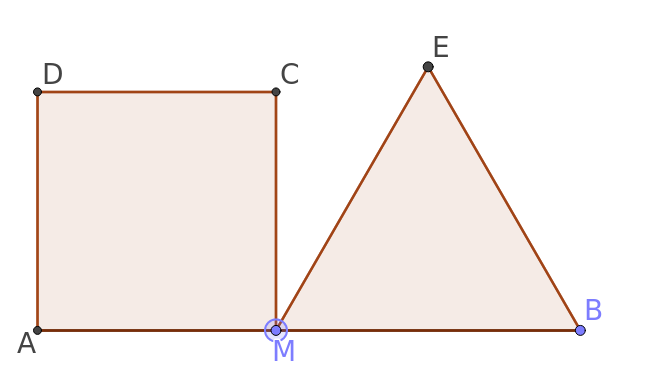
\includegraphics[width=0.3\textwidth]{image/calcul/pbtricar2.png}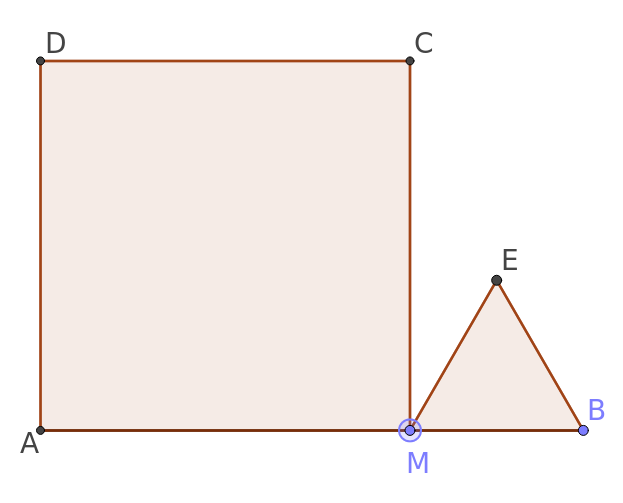
\includegraphics[width=0.3\textwidth]{image/calcul/pbtricar3.png}

	\emph{Début de la réponse.}
	Notons $d$ la distance $AM$. Le périmètre du carré mesure $P_c=4\times AM=4\times d = 4d$. 
	Notons $d'$ la distance $MB$. Le périmètre du triangle mesure $P_t=3\times MB = 3\times d'=3d'$. Mais on a $d+d'=1$ donc nécessairement, $d'=1-d$. Ainsi, $P_t=3\times(1-d)$. Pour égaliser les périmètres, il suffit d'écrire que $P_c=P_t$. En substituant avec les expressions trouvées, il faut donc placer le point $M$ à la distance $d$ du point $A$, où le nombre $d$ vérifie l'égalité suivante :
	\begin{equation}
		4d=3(1-d).
	\end{equation}
	Cette égalité dans laquelle figure un nombre inconnu représenté ici par la lettre $d$ s'appelle une {\bfseries équation}. On appelle \emph{résoudre une équation} l'action de trouver tous les nombres inconnus qui réalisent cette égalité.

	\paragraph{Problème B} Un automobiliste se déplace avec une vitesse $v$ pour parcourir une distance $d$ (par exemple, un chauffard roule à $v=$160km/h pour faire Paris-Toulouse en voiture, $d\approx 630$km). Quelle sera la durée du trajet\,?

	\emph{Début de la réponse.}
	On sait que la vitesse est la proportion de distance parcourue par rapport à un temps donné : si pendant une même durée je parcours une plus grande distance, alors je vais plus vite\,; de même, si je parcours la même distance pendant une durée plus courte, alors je vais plus vite. Ainsi, un mobile qui parcourt la distance $d$ pendant la durée $d$, a une vitesse qui vérifie l'égalité suivante\,:
	\begin{equation}
		v=\frac{d}{t}.
	\end{equation}
	Dans le problème B, la vitesse et la durée sont données, et nous cherchons la durée. Il s'agit d'isoler la durée et de l'exprimer en fonction des deux autres grandeurs, on aimerait secouer cette équation jusqu'aboutir à quelque chose de la forme \og{}$v=\ldots$\fg. 

\chapter{Théorie du produit en croix}\label{chap_croix}
	\section{(R)appel : classe d'équivalence}
		\initial{L}{a} mathématique, c'est la théorie abstraite des relations entre des quantités (par \guil{quantité} j'entends évidemment les nombres, mais aussi des objets potentiellement plus abstraits qui généralisent les nombres, ou même, des objets géométriques). La notion de relation en mathématiques est donc fondamentale. La relation la plus utile et la plus simple, c'est l'égalité. Mais il y en a d'autres. Par exemple, le parallélisme entre deux droites est aussi une relation entre deux objets. Bref, tout n'est que relation univoque entre objets dans cette discipline. Mais une relation sans contenu est vide. Donc, on commence toujours par décrire l'espace général dans lequel on travaille afin de savoir de quoi on parle, avant d'en parler. Par exemple : est-ce qu'on travaille avec des objets géométriques dans le plan d'Euclide, est-ce qu'on travaille sur des nombres\,? et bien d'autres cas possibles. Pour généraliser tout cela, on peut noter cet \guil{espace général} comme un ensemble $E$ qui contient des éléments $a$, $b$, $c$, etc. La plupart des \guil{phrases} écrites en symboles mathématiques commenceront donc par \guil{$\forall a, b, c,\ldots \in E,\ldots$} ce qui peut se traduire par\footnote{en guise de rappel, micro-dico\,: $\forall=$\guil{pour tout}, $\wedge=$\guil{et}, $\lor=$\guil{ou} (inclusif), $\in$=\guil{appartient à} ou \guil{appartenant à} ou autre conjugaison, selon le contexte, .} \guil{pour tous $a$, $b$, $c$ et éventuellement autres éléments appartenant à l'ensemble $E$, on a\ldots}.

		Ainsi, si par exemple l'on travaille dans l'ensemble des nombres entiers naturels $\N$, on aura $E=\N$, et ses éléments seront les nombres entiers. Dans le cas général, si l'on note une relation générique $R$, alors on dit que deux éléments $a$ et $b$ dans l'ensemble $E$ sont en relation $R$ en notant tout simplement $aRb$. Si l'on veut dire que $R$ est l'égalité, et qu'on remplace $a$ par $1+1$ et $b$ par $2$, alors la phrase \guil{$aRb$} devient tout simplement \guil{$1+1=2$}. On peut aussi penser à la relation \guil{strictement inférieur}, notée $<$. Si l'on remplace $a$ par $1$ et $b$ par $2$, on obtient tout simplement la phrase \guil{$1<2$}.

		\begin{defi}
			Soit $R$ une relation dans un ensemble $E$. On dit que $R$ est une relation d'équivalence lorsque elle vérifie les propriétés suivantes\footnote{Exercice\,: traduire en français les trois points de la définition\,!}\,:
			\begin{itemize}[$\bullet$]
				\item Réflexivité\,: $\forall a\in E, aRa$.
				\item Symmétrie\,: $\forall a,b\in E, aRb\Rightarrow bRa$.
				\item Transitivité\,: $\forall a,b,c\in E, (aRb\wedge bRc)\Rightarrow aRc$. 
			\end{itemize}
		\end{defi}

		On peut vérifier très rapidement que l'égalité est bien une relation d'équivalence. Mais c'est aussi vrai pour le parallélisme (en admettant que deux droites identiques constituent un cas particulier de droites parallèles). Pour ceux qui ont suivi le cours sur le théorème de Thalès : la semblabilité de triangles (et donc de figures géométriques) est une relation d'équivalence. En revanche, la relation $<$ n'est pas une relation d'équivalence. En effet, on a $1<2$ mais on ne peut pas les échanger\,: $2<1$ est faux. Donc la réflexivité est contredite.


		\begin{defi}
			Soit $R$ une relation d'équivalence dans un ensemble $E$ et soit $e\in E$. La classe d'équivalence qui a pour représentant $e$, souvent notée $\bar{e}$, est l'ensemble des éléments qui sont en relation avec $e$. On note de manière compacte\,:
			\begin{equation}
				\bar{e}=\{x\in E | eRx\}.
			\end{equation}
		\end{defi}


		Ici, l'égalité perd un peu son intérêt, car il y a identité entre le représentant d'une classe et sa classe elle-même. En effet, l'ensemble des nombres égaux à 2, c'est... 2. Le parallélisme offre quelque chose de plus intéressant. En effet, si l'on se donne une droite, il existe une infinité de droites qui lui sont parallèles, et elles recouvrent même l'intégralité du plan. La classe d'équivalence de toutes ces droites, en fait, donne la notion de \emph{direction}\,: c'est en quelque sorte le degré d'inclinaison de la droite dans le plan, qui est commun à toute cette infinité de droites.

		%Remarque\,: parfois, pour éviter des ambiguïtés, on note $e/E$ au lieu de $\bar{e}$, afin de savoir dans quel ensemble global se place la classe d'équivalence. En effet, si l'ensemble $E$ est contenu dans l'ensemble $F$, alors $e/E$ n'est pas nécessairement la même chose que $e/F$, et alors la notation $\bar{e}$ pourrait présenter une ambiguïté. Exemple : si l'on considère une droite, selon que l'on considère cette même droite appartenant à un plan ou appartenant à l'espace à trois dimensions, alors on comprend bien que la classe d'équivalence du parallélisme dont le représentant est cette droite n'est pas la même, selon que l'on est dans le plan ou dans l'espace.


	\section{Fondements de la théorie}\label{sec_fond}
		La théorie du produit en croix que je propose est en opposition totale avec le vomi académique qui propose de retenir des recettes magiques de calculs de \guil{quatrième proportionnelle} à l'aide de signes sataniques sortis du chapeau du professeur. Nous allons proposer une théorie axiomatique puis déductive du produit en croix. Il s'agit simplement de définir les fractions comme représentants d'une classe d'équivalence, le quotient de deux nombres --- c'est-à-dire le résultat de leur division.
		\begin{axi}[Loi du produit en croix]
			Soient $a$, $b$, $c$, et $d$ quatre nombres (réels). Alors\,:
			\begin{equation}
				\boxed{\frac{a}{b}=\frac{c}{d} \Leftrightarrow ad=bc}
			\end{equation}
			Autrement dit, si $a$ et $b$ sont deux nombres, on définit le quotient $\frac{a}{b}$ comme la classe d'équivalence des couples de nombres $(c;d)$ tels que $ad=bc$. En langage plus formel, si $\mathbb{E}$ est un ensemble de nombre, on écrit, sous réserve d'existence\,:
			\begin{equation}
				\frac{a}{b}=\left\{ (c,d)\in\mathbb{E}^2|ad=bc\right\}			
			\end{equation}
		\end{axi}

		\begin{rema}
			À ce stade nous ne nous soucions pas de la division par zéro (nous démontrons plus loin que zéro n'a pas d'inverse). En effet, à ce stade, d'après l'axiome, pour tous nombres $a$ et $b$, $\frac{a}{0}=\frac{b}{0}$, quoique cela veuille dire.
		\end{rema}

		Toute cette artillerie lourde peut vous paraître compliquée à comprendre en première lecture. Nous allons expliciter cet axiome avec différents niveaux de lecture.
		\begin{enumerate}
			\item Niveau 0. \\ Déjà, il s'agit d'un axiome. Nous ne le démontrerons pas. Il s'agit du point de départ de notre théorie. 
			\item Niveau 1. \\ Pour passer de gauche à droite dans l'égalité de l'axiome, on constate que l'on a écrit le produit des nombres aux extrémités d'une croix qui remplacerait le signe égal. On pourrait donc renommer cet axiome\,: égalité des produits croisés. D'où le fameux nom \guil{produit en croix}.
			\item Niveau 2. \\ Ce qu'il faut comprendre, c'est que $q=a/b$ est le résultat de la division de $a$ par $b$. On peut démontrer à partir de l'axiome que $q$ est l'unique nombre véfifiant $qb=a$. En effet, puisque diviser par 1 ne change pas le résultat, on peut écrire que $q/1=a/b$, et en appliquant l'axiome, on trouve que $qb=a\times1=a$. Réciproquement, s'il existait $q$ et $q'$ qui vérifiaient l'égalité $qb=a$, en remarquant que $a=a\times 1$, on trouve que $q/1=a/b=q'/1$ et donc que $q=q'$\,; le résultat de la division de $a$ par $b$ est donc bien unique grâce à cet axiome.
			\item $(\star)$ Niveau 3. La notion de classe d'équivalence permet de faire une distinction entre le quotient et la fraction. Le quotient est un nombre, c'est le résultat unique d'une division. Mais cette division en tant qu'opération n'est pas unique. Ainsi, la fraction apparaît comme une écriture possible du quotient. Lorsque l'on écrit par exemple $2/3$ en tant qu'écriture, on laisse l'opération en attente, sans l'effectuer. Et donc $2/3$ en tant que fraction n'est pas égale à $4/6$. Mais si on considère $2/3$ en tant que quotient, alors on sous-entend que même si le résultat de l'opération de division n'est pas explicitement écrit, il est sous-entendu par l'écriture. Et alors, on peut bien écrire que $2/3=4/6$, les quotients précédents étant considérés en tant que nombres. D'ailleurs, on peut utiliser l'axiome pour vérifier cette égalité\,: en effet, on a bien $2\times6=3\times4$. Ici on a écrit que $2/3=4/6$, mais en vérité il y a une infinité de quotients qui sont égaux à $2/3$\,: $4/6;\;6/9;\;8/12;$ etc. Bref, l'ensemble de toutes les fractions $c/d$ où les nombres $c$ et $d$ ont été choisis de manière à ce que $2\times d=3\times c$.  
		\end{enumerate}

		$(\star)$ \emph{Jusqu'à la section \ref{sec_regles}, ce qui suit peut être sauté en première lecture.}

		À titre de remarque préliminaire, une fois que l'on a défini le quotient, il convient de définir l'inverse d'un nombre.
		\begin{defi}
			Soit $a$ un nombre. Sous réserve d'existence, $b$ est un inverse de $a$ si $a\times b=b\times a=1$. On notera alors $b=1/a$.
		\end{defi}
		\begin{thm}
			L'inverse d'un nombre est unique.
		\end{thm}
		\begin{proof}
			Soient $b$ et $b'$ deux inverses de $a$. Alors $ab=ab'=1$. D'après l'axiome, on a $b=1/a=b'$.
		\end{proof}
		\begin{cor}
			Diviser par un nombre revient à multiplier par son inverse.
		\end{cor}
		\begin{proof}
			Supposons que $q=\frac{a}{b}$, alors $qb=a$. Considérons le nombre $a\times1/b$. Alors on a $a\times 1/b\times b=a\times 1 =a$ car multiplier par $b$ est l'opération réciproque de diviser par $b$. Par unicité du quotient, on a bien $a/b=a\times 1/b$.
		\end{proof}

		Souvent, vos professeurs de mathématiques vous ont hurlé dessus ou ont eu des crises cardiaques lorsque vous avez divisé un nombre par zéro. Le théorème suivant explique pourquoi.
		\begin{thm}
			0 n'a pas d'inverse.
		\end{thm}
		\begin{proof}
			Si zéro avait un inverse, alors il existerait un nombre $x$ tel que $0\times x=1$, mais pour tout nombre $x$, $0\times x=0$ et donc on aurait $1=0$, ce qui est absurde.
		\end{proof}


	\section{Quelques règles de calcul utiles}\label{sec_regles}
		Voici quelques règles de calculs fort utiles pour manipuler des expressions algébriques\,:
		\begin{thm}
			Soient $a$,$b$,$c$,$d$ des nombres tels que les dénominateurs apparaissants plus bas soient non nuls. Alors les opérations élémentaires s'effectuent de la manière suivante\,:
			\begin{itemize}[$\bullet$]
				\item simplification des fractions\,:
				\begin{equation}
					\frac{a}{b}=\frac{a}{b}\times\frac{d}{d}=\frac{ad}{bd};
				\end{equation}
				\item multiplication d'un quotient par un nombre\,:
				\begin{equation}
					\frac{a}{b}\times c=\frac{ac}{b};
				\end{equation}
				\item multiplication et division de deux quotients\,:
				\begin{equation}
					\frac{a}{b}\times\frac{c}{d}=\frac{ac}{bd};\quad \frac{\frac{a}{b}}{\frac{c}{d}}=\frac{a}{b}\times\frac{d}{c}=\frac{ad}{bc};
				\end{equation}
				pour la dernière série d'égalités, on remarque que diviser par un nombre revient à le multiplier par son inverse. Notamment\,:
				\begin{equation}
					\frac{\frac{a}{b}}{c}=\frac{a}{b}\times\frac{1}{c}=\frac{a}{bc};
				\end{equation}
				\item addition ou soustraction de deux quotients, selon qu'ils aient ou non le même dénominateur\,:
				\begin{equation}
					\frac{a}{b}\pm\frac{c}{b}=\frac{a\pm c}{b};\quad \frac{a}{b}\pm\frac{c}{d}=\frac{ad\pm bc}{bd}.
				\end{equation}
			\end{itemize}
		\end{thm}
		\begin{proof}
			Ce sont des démonstrations élémentaires du même type que les démonstrations de la section \ref{sec_fond} (ah\,! je vois déjà les petits malins qui ont sauté les passages difficiles\,! Vous voilà bien embarrassés maintenant.). Elles sont amusantes à faire, à petite dose. C'est la raison pour laquelle je les laisse en exercices. Si vous êtes capables d'en faire quelques unes, cela signifie que vous avez compris la méthode, ce qui est le plus important.
		\end{proof}

		Remarque : pour la dernière égalité du théorème, en pratique il s'agit de réduire les deux fractions à ajouter/soustraire au même dénominateur afin de pouvoir effectuer l'opération avec les numérateurs. En général on ne va pas utiliser exactement cette égalité, mais on va simplifier directement en cherchant le diviseur commun le plus grand entre les deux dénominateurs\footnote{($\star$) En fait, tout ceci pourrai s'écrire formellement ainsi\,:
		\begin{equation}
			\frac{a}{b}\pm\frac{c}{d}=\frac{\frac{ad}{\mathrm{pgcd}(b,d)}\pm \frac{cb}{\mathrm{pgcd}(b,d)}}{\mathrm{ppcm}(b,d)}
		\end{equation}.}. Prenons un exemple\,:
		\begin{equation}
			\frac{1}{6}-\frac{2}{9}=\frac{1\times 3}{6\times 3}-\frac{2\times 2}{9\times 2}=\frac{3}{18}-\frac{4}{18}=-\frac{1}{18}.
		\end{equation}

		À présent, il convient de résoudre un problème classique. Imaginons que sur les quatre nombres $a$, $b$, $c$, $d$, trois soient donnés et qu'on cherche le quatrième, sachant que $a/b=c/d$. C'est ce qu'on appelle le problème du produit en croix. Je pourrais donner un théorème général qui donnerait toutes les solutions possibles, mais il est plus intéressant que le lecteur cherche lui-même la solution.


	\paragraph{Exercices}
	\begin{enumerate}
		\item Résoudre les équations suivantes (trouver le nombre inconnu en fonction des nombres connus) : $\frac{1}{x}=\frac{2}{3}$ ; $\frac{3}{4}=\frac{2}{y}$. Pour procéder, on utilisera d'abord l'axiome du produit en croix, puis on divisera les deux membres de l'égalité par le nombre qui multiplie l'inconnue afin de s'en débarrasser par simplification d'une fraction.

		\item On suppose que $\frac{a}{b}=\frac{c}{d}$. Exprimer chacun des quatre nombres en fonction des trois autres\footnote{Cela signifie qu'on veut écrire\,: $a=\ldots$, puis $b=\ldots$, etc. où les points de suspension contiennent une expression qui dépendent des trois autres nombres que celui à gauche du signe égal.}.

		\item Résoudre le problème B.
	\end{enumerate}

	\emph{Solutions\,:}
	\begin{enumerate}
		\item $\frac{1}{x}=\frac{2}{3} \Leftrightarrow 1\times 3 = 2\times x$ d'après l'axiome. En simplifiant, on écrit donc que $2x=3$. Mais on ne cherche pas $2x$, on cherche $x$. Ainsi, puisqu'on a $2$ fois trop de $x$, on va diviser les deux côtés de l'égalité par 2 (afin de ne pas déséquilibrer l'égalité). Ce qui donne donc\,: $\frac{2x}{2}=\frac{3}{2}$. Mais d'après la règle de simplification des fractions, on a simplement $x=\frac{3}{2}$. Et donc la solution est $\frac{3}{2}$. 

		En général, on ne s'embarrasse pas d'une rédaction aussi lourde. Pour résoudre la deuxième, on écrira utilement\,:
		\begin{equation}
			\frac{3}{4}=\frac{2}{y} \Leftrightarrow 3\times y = 2\times 4 \Leftrightarrow \frac{3y}{3}=\frac{8}{3} \Leftrightarrow y=\frac{8}{3} \nonumber
		\end{equation}
		et donc la solution est $8/3$.

		Avec un peu de pratique, on peut même le faire en une étape, "de tête".

	\item Avec la même méthode, on peut trouver que $\frac{a}{b}=\frac{c}{d}\Leftrightarrow a=\frac{bc}{d}$. Les autres sont laissées au lecteur.
	\item On trouve $t=d/v$, et si on remplace par les valeurs, on trouve donc $t=630$(km)$/160$(km/h)$\approx 4$h.

	\end{enumerate}
	
\chapter{Équations du premier degré}\label{chap_eqp}
	\section{Résolution algébrique pure}
		On parle de premier degré lorsque l'inconnue (par exemple $x$) intervient en quelque sorte directement dans l'équation\,: soit multipliée par un nombre, soit toute seule. Cependant, on n'admettra pas que l'inconnue apparaisse sous la forme $x\times x$ ou sous la forme $1/x$. En fait, on peut montrer que toutes les équations du premier degré peuvent se mettre sous la forme $ax+b=0$ où $a$ et $b$ sont des nombres quelconques. 

		\begin{axi} (Conservation des quantités)
			Pour tous nombres $a$, $b$, et $c$,
			\begin{equation}
				a+b=c \Leftrightarrow a=c-b.
			\end{equation}
			Autrement dit, si à deux quantités égales, on ajoute ou on retranche la même quantité, alors les résultats obtenus seront égaux.\item{On trouve cet axiome dans l'ouverture des \emph{Éléments} d'Euclide.}
		\end{axi}

		On rappelle que par convention, $ab+c=(ab)+c$. Dans les livres communs de l'enseignement secondaire, on appelle cela la \emph{priorité de la multiplication (ou de la division) sur l'addition (ou la soustraction)}. Nous préférons dire, comme Stella Baruk, que le nombre $(ab)+c$ est globalement une somme\,: la somme de $ab$ et de $c$. Autrement dit, l'opération globale à effectuer est une addition. L'addition donc l'opération qu'il faudra effectuer en dernier, une fois qu'on aura intégralement déterminé ses termes à additionner, $ab$ et $c$. 


		\begin{exo}
			Résoudre les équations suivantes, c'est-à-dire, trouver le nombre inconnu (désigné par une lettre) qui réalise l'égalité.
			\begin{enumerate}
				\item Ceinture rose
				\begin{equation}
				 	x+1=2;\quad 2y=4;\quad 2y+3=5.
				\end{equation} 
				\item Ceinture blanche
				\begin{equation}
					5z-2=3;\quad 2u-1=9.
				\end{equation}
				\item Ceinture jaune
				\begin{equation}
					3u-2=0;\quad 3v+2=0
				\end{equation}
				\item Ceinture verte
				\begin{equation}
					2w+5=5w-4
				\end{equation}
				\item Ceinture rouge
				\begin{equation}
					\frac{2}{3}x-\frac{5}{6}=-\frac{9}{11}x+\frac{7}{13}
				\end{equation}
			\end{enumerate}
		\end{exo}
	\section{Approfondissement\,: résolution dans un ensemble}

		Nous déjà avons vu quelques ensembles de nombres\,: $\N$, $\Z$, $\D$, et $\Q$ (voir annexe \ref{app_nbs} pour des rappels).
		En fait, lorsqu'on cherche à résoudre une équation, on cherche un nombre dans un ensemble défini à l'avance. Ce point est d'une très grande importance car cela peut changer l'existence ou non d'une solution. Voici un petit exemple/contre-exemple très classique\,:
		Résoudre l'équation suivante sachant que $x\in \N$ : $2x=1$. En divisant par deux cette égalité, on trouve que
		\begin{equation}
			2x=1 \Leftrightarrow x=\frac{1}{2} 
		\end{equation}

		Cette ligne signifie : \guil{dire que $2x=1$ est équivalent à dire que $x=1/2$}. C'est un raisonnement par équivalence. Cependant, dire qu'une proposition équivaut à une autre ne veut pas dire que l'une ni l'autre soit vraie. Surtout si l'on se rappelle qu'on avait exigé que $x$ soit un nombre entier naturel. En effet, $2x=1$ c'est la même chose que $x=1/2$, soit $0.5$ en écriture décimale. Mais ceci entre en contradiction avec l'exigence de départ : que $x$ soit un entier naturel. Ainsi, puisque l'équation équivaut à quelque chose d'impossible (que $x=0.5$ \emph{et en même temps} que $x\in\N$), alors on concluera que l'équation n'a pas de solution dans $\N$. On écrira alors que l'ensemble des solutions, noté $S$ par convention, est vide. Cet ensemble est représenté par le symbole $\emptyset$ en mathématiques. Voici donc comment on rédige tout ce raisonnement en symboles mathématiques\,:
		\begin{equation}
		 	2x=1\Leftrightarrow x=\frac{1}{2}=0.5\notin\N ; \quad S=\emptyset.
		\end{equation} 
		En revanche, si l'on souhaite résoudre cette équation dans un ensemble de nombres plus \guil{gros}, par exemple l'ensemble des nombres décimaux, alors on écrira\,:
		\begin{equation}
		 	2x=1\Leftrightarrow x=\frac{1}{2}=0.5\in\D ; \quad S=\{0.5\}.
		\end{equation} 
		J'attire votre attention sur la notation $S=\{0.5\}$\,: $S$ n'est pas un nombre, c'est un ensemble de nombres, celui qui contient le nombre $0.5$. Cela sera utile lorsque certaines équations contiendront plus qu'une seule solution. 
		Nous alons en construire une immédiatement. Nous avons besoin d'un théorème\,:
		\begin{thm}
			Un produit de facteurs est nul si et seulement si au moins l'un des facteurs est nul. Autrement dit, si $a,b,c,\ldots$ sont des nombres, alors\,:
			\begin{equation}
				abc\ldots = 0 \Leftrightarrow(a=0\lor b=0 \lor c=0\lor \ldots).
			\end{equation}
		\end{thm}

		\begin{proof}
			$\Leftarrow$ immédiat par propriété de la multiplication par zéro.

			$\Rightarrow$ raisonnement par contraposée. Si aucun des facteurs n'est nul, alors leur produit est non nul.
		\end{proof}

		Ainsi, résolvons par exemple dans $\R$ l'équation $(x+1)(x-1)=0$. On écrira\,:
		\begin{equation}
			(x+1)(x-1)=0 \Leftrightarrow (x+1=0\lor x-1=0) \Leftrightarrow (x=-1\lor x=1); \quad S=\{1;-1\}.
		\end{equation}
		(Nous n'avons pas précisé qu'ici, $1$ et $-1$ sont des nombres réels car cela ne présentait pas d'ambiguïté). Ici, l'ensemble solution est un ensemble qui contient non pas un, mais deux nombres. 

		Voyons un cas encore plus tordu. Essayons de résoudre, par exemple dans l'ensemble $\Q$, l'équation $r=r$. En fait, cette égalité est vraie pour tout nombre rationnel $r$, donc tous les nombres de l'ensemble $\Q$ sont solutions. L'ensemble solution n'est autre que $\Q$ lui-même\,: $S=\Q$\,!

		Et tentons de résoudre $z=z+1$ dans l'ensemble $\R$. Avec un peu d'intuition, on peut voir qu'il n'existe aucun nombre $z$ vérifiant cette égalité, mais une fois n'est pas coutûme, faisons les automathes avec un raisonnement par l'absurde\,: supposons qu'il existe un nombre réel $z$ qui vérifie l'égalité escomptée. Alors, en soustrayant $z$ des deux côtés, on obtient\,: $z-z = z+1-z$, et en simplifiant, on obtient\,: $0=1$. Cette égalité étant absurde, nous devons contredire l'hypothèse qui y a menée, et donc, il n'y a pas de solution\,: $S=\emptyset$.






\chapter{Résolution graphique des équations}

	\section{Repère cartésien}
		Descartes a démocratisé le lien entre la géométrie et l'algèbre, avec ce qu'on appelle aujourd'hui les \emph{repères cartésiens}. Nous allons  présenter le repère le plus utile qui soit, le repère cartésien orthogonal. Nous utiliserons une présentation semi-intuitive comme celle de Descartes\footnote{La théorie axiomatique des nombres réels sera abordée dans une future leçon.}.

		Considérons une droite. Plaçons un point arbitraire $O$ sur cette droite, ainsi qu'un autre point arbitraire nommé $I$. Le premier point sera appelé {\bfseries l'origine} du repère alors que le deuxième point permettra de définir {\bfseries l'unité de mesure des distance}. En effet, nous venons de créer une unité de mesure, et nous poserons que la distance $OI$ sera égale à l'unité.
		Une telle droite a plusieurs noms dans les livres de mathématiques; pour l'heure nous la nommerons \emph{droite graduée}.

		Plaçons un point $A$ de manière arbitraire sur la droite. Nous allons définir de manière unique un nombre qui permettra de repérer ce point sur la droite. Ce nombre, souvent noté $x$, est l'abscisse du point $M$. Il est défini comme suit\,:
		\begin{itemize}[$\bullet$]
			\item Si $M$ est du même côté que\footnote{La notion \guil{du même côté que} sera définie formellement dans le chapitre de trigonométrie.} $I$ par rapport à $O$, $x=\frac{OM}{OI}$ (illustration ci-dessous).

			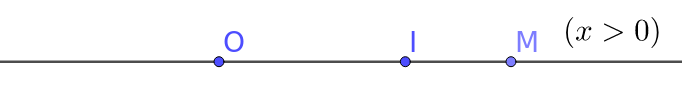
\includegraphics[width=0.6\textwidth]{image/calcul/point1d1.png}
			\item Sinon, $x=-\frac{OM}{OI}$ (illustration ci-dessous). 

			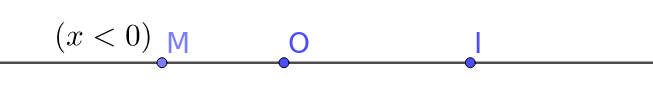
\includegraphics[width=0.6\textwidth]{image/calcul/point1d2.png}
		\end{itemize}



		En deux dimensions, il faut ajouter un deuxième axe qui coupe le premier. Le plus simple est de prendre un axe perpendiculaire au premier, qui le coupe en $O$. Ensuite, nous choisissons un point $J$ tel que $OI=OJ$ pour avoir la même unité de mesure dans les deux axes\footnote{Ce n'est pas une obligation. Les deux axes pourraient même avoir des origines différentes. Mais nous commençons par présenter le cas le plus simple.}. Un tel repère est appelé \emph{Repère orthonormé}. Si nous choisissons de mettre le point $I$ \guil{vers la droite} et le point $J$ \guil{vers le haut}, on dit que le repère est \emph{direct}, sinon il est \emph{indirect}\footnote{Il s'agit de l'orientation du repère. Plus rigoureusement\,: si les points $O$, $I$, $J$, dans cet odre, tournent dans le sens anti-horaire, alors le repère est direct. Sinon il est indirect. L'orientation sera définie formellement dans le chapitre de trigonométrie.}. Ayant construit une deuxième droite graduée, on peut y placer un autre point, $B$ également repréré par une autre abscisse, le nombre $y$. Mais en général, pour le deuxième axe, on préfère parler d'\emph{ordonnée} plutôt que d'abscisse, afin d'éviter de confondre les deux. 
		Muni de ces deux nombres $(x,y)$, on peut construire un point du plan, le point $M$, qui sera l'unique point tel que $OAMB$ est un rectangle. 

		Réciproquement, si l'on se donne un point du plan $M$, alors on pourra trouver de manière univoque son abscisse $x$ et son ordonnée $y$. Pour ce faire, il suffit de tirer la droite perpendiculaire à $(OI)$ passant par $M$\,; cette droite coupe $(OI)$ en $A$ et $x$ n'est autre que l'abscisse de $A$. De même pour $y$ en prenant la perpendiculaire à $(OJ)$ passant par $M$.

		Les nombres $(x,y)$ regroupés dans un couple sont les {\bfseries coordonnés cartésiennes} du point $M$.

		Nous  illustrons cela ci-dessous\,:

		\vspace{0.2cm}

		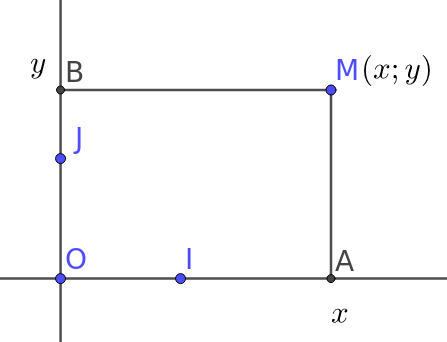
\includegraphics[width=0.4\textwidth]{image/calcul/point2d.png}			

		Notez que d'après le théorème de Pythagore, si le point $M$ est repéré par les coordonnées $(x,y)$ et $N$ par les coordonnées $(x',y')$, alors la distance $MN$ se calcule ainsi\,:
		\begin{equation}
			MN=\sqrt{(x-x')^2+(y-y')^2}
		\end{equation}

		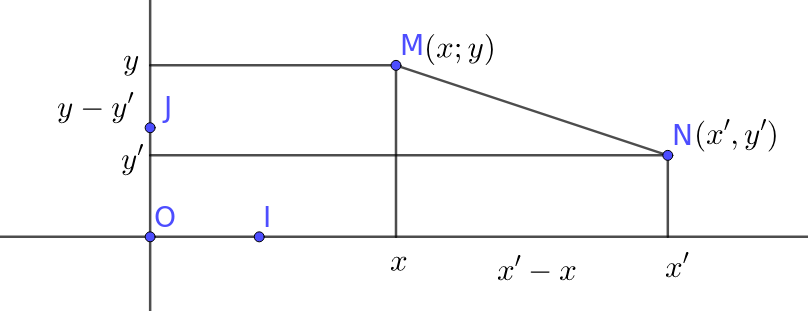
\includegraphics[width=0.7\textwidth]{image/calcul/point2dpyth.png}


	\section{Courbe d'une fonction}
		Maintenant que nous savons repérer un point quelconque dans le plan, imaginons que nous fassions varier $x$ et $y$ continument dans le temps. Imaginons que le point $M$ soit au préalable plongé dans de l'encre et qu'il laisse une trace. Alors le résultat sera une ligne tracée sur le plan, que l'on a coutûme d'appeler \emph{courbe}\footnote{Bien qu'elle ne soit pas forcément courbée. Ainsi, les droites sont aussi des \guil{courbes}\,!}. Il existe de nombreuses façons de construire des courbes et nous ne les aborderons pas toutes. La manière la plus simple de construire des courbes est de considérer que les quantités $x$ et $y$ ont une relation de dépendance, et en particulier, que $y$ dépend de $x$. On écrira que $y=f(x)$, sous-entendu, que $y$ est fonction de $x$. Notez que $f(x)$ se lit \guil{$f$ de $x$} (le choix de la lettre $f$ correspond au mot \guil{fonction}, mais il est possible de prendre n'importe quelle autre lettre). De là, il suffit de faire varier le nombre $x$ et, pour chaque valeur connue de $x$, il suffit de calculer le nombre $y$ correspondant. On obtient un tableau qui regroupe de nombreuses coordonnées du point mobile, et il suffit de les tracer et de les relier plus ou moins continument pour obtenir quelque chose qui ressemble à une courbe.

		Essayons par exemple de tracer la courbe dont les coordonnées vérifient $y=x^2$. Ici, nous avons donc $c(x)=x^2$ (le choix de la lettre $c$ vient du fait que le processus de cette fonction consiste à élever le nombre $x$ en son carré, $x^2$). En théorie, $x$ varie de moins l'infini jusqu'à plus l'infini, mais la taille du papier n'étant pas infinie, nous allons restreindre le domaine de variation du nombre $x$. Nous partirons de $x=-2$ et nous irons jusqu'à $x=+2$ par exemple. Alors, il faut remplir le tableau suivant\,:

		\begin{tabular}{|c|c|c|c|c|c|c|c|c|c|c|}
			\hline
			$x$     &$  -2 $&$ -1.8 $&$ -1.6 $&$ -1.4 $&$ -1.2 $&$ -1 $&$ -0.8 $&$ -0.6 $&$ -0.4 $&$ -0.2 $\\
			\hline
			$y=x^2$ &       &         &       &        &        &      &         &       &         &        \\
			\hline
		\end{tabular}

		\vspace{0.3cm}

		\begin{tabular}{|c|c|c|c|c|c|c|c|c|c|c|c|}
			\hline
			$x$     &$  0 $&$ 0.2    $&$ 0.4 $&$ 0.6  $&$ 0.8  $&$ 1   $&$1.2    $&$ 1.4 $&$ 1.6   $&$ 1.8  $& 2\\
			\hline
			$y=x^2$ &       &         &       &        &        &      &         &       &         &        & \\
			\hline
		\end{tabular}

		Pour la première case vide, il faut effectuer le calcul suivant en remplaçant $x$ par la valeur annoncée\,: $y=x^2=(-2)^2=(-2)\times(-2)=+4$. Et ainsi de suite pour toutes les autres cases. Souvent, on utilise des logiciels pour automatiser la procédure. Geogebra le fait automatiquement, et calcule beaucoup plus de valeurs que dans ce simple tableau, ce qui donne l'illusion d'une belle courbe continue. Nous, nous allons utiliser le tableur\,:

		\noindent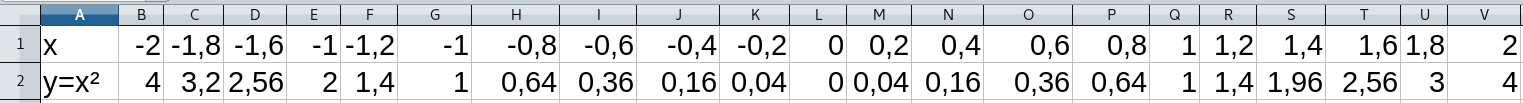
\includegraphics[width=\textwidth]{image/calcul/valfctcar.png}

		Pour obtenir ce tableau, il suffit de rentrer -2 en B1, puis de rentrer en C1\,: \mintinline{python}{=B+0,2} et d'étendre jusqu'à ce qu'on atteigne le nombre 2. Ensuite, il suffit de rentrer en B2 la formule\,: \mintinline{python}{=B1*B1} et d'étendre.

		Nous obtenons alors le \emph{tableau de valeurs de la fonction carré}. Pour tracer ceci, il faut placer chaque couple abscisse/ordonnée dans le plan. Par exemple, lorsque $x=2$, on a $c(x)=4$. Ainsi, il faudra placer un point dont les coordonnées sont $(2;4)$. On fait de même avec les autres points, ce qui donne une idée du graphe de la courbe.

		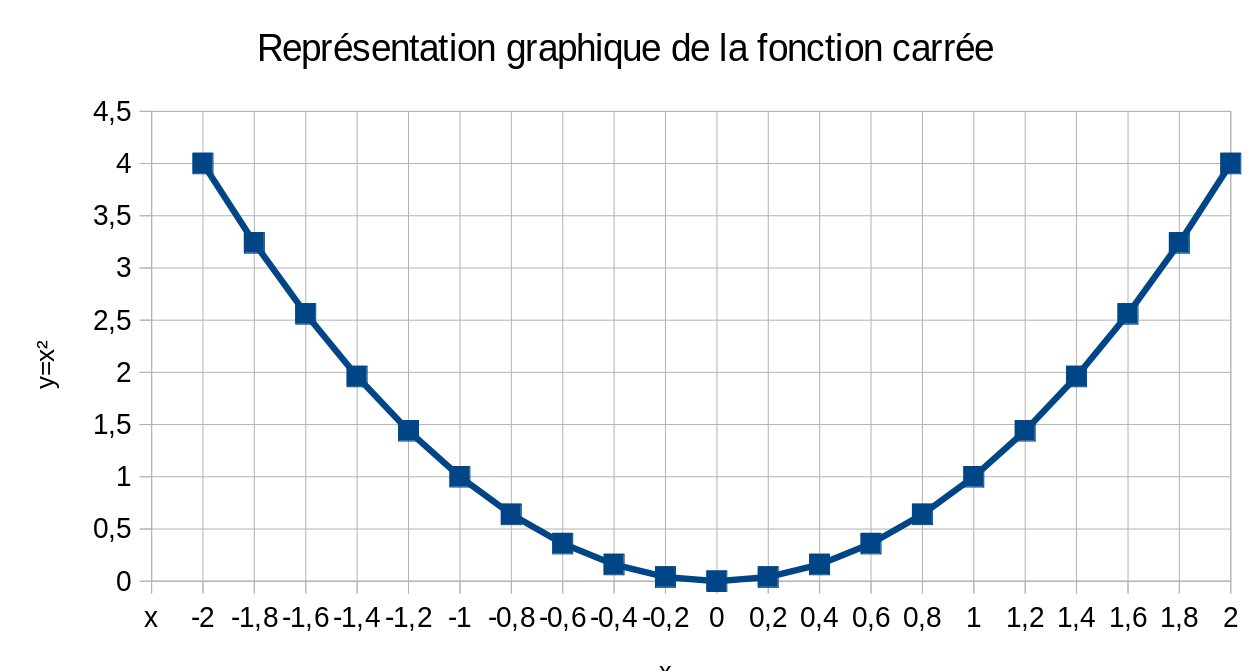
\includegraphics[width=0.9\textwidth]{image/calcul/courbe_fct_car.png}

	\section{Modélisation et résolution graphiques d'une équation}

		Une équation du premier degré d'inconnue $x$ peut toujours se mettre sous la forme $f(x)=g(x)$ où $f(x)=ax+b$ et $g(x)=cx+d$ où $a$, $b$, $c$, et $d$ sont des nombres fixés. Si on n'aime pas le calcul, il suffit de tracer les graphes des fonctions $f$ et $g$ et de visualiser où les courbes se coupent. Lorsqu'il y a une unique solution, on a affaire à des droites qui se coupent en un point de coordonnées $(x;y)$. L'abscisse $x$ de ce point est la solution de cette équation. Il suffit donc de lire l'abscisse du point solution sur l'axe des abscisse.

		\begin{exo}
			On considère une voiture sur une autoroute rectiligne se déplaçant à la vitesse $v=130$km/h. On modélise la route par une droite graduée d'origine $O$. La droite est orientée dans le sens du mouvement de la voiture. On note $x(t)$ l'abscisse de la voiture à la date $t$ ; ce nombre représente la position de la voiture sur la droite. On suppose qu'à $t=0$, la voiture passe par $O$.
			\begin{enumerate}
				\item Démontrer que $x(t)=v t$.
				\item Convertir $v$ en m/s.
				\item Compléter le tableau suivant\,:

				\begin{tabular}{c|c|c|c|c|c|c|c|c|c|c|c}
					t (s) & -5 & -4& -3& -2& -1& 0& 1& 2& 3& 4& 5 \\
					\hline
					x(t) (m)& &   &   &    &   &  &  &  &  &  &  
				\end{tabular}

				\item Tracer le graphe de la fonction $x:t\mapsto x(t)$. Commenter cette courbe. Y avait-il besoin d'autant de points que de colonnes dans le tableau précedent pour tracer la courbe\,?
				%\item Calculer l'angle que fait la courbe avec l'axe des abscisses.
				\item Une autre voiture se déplace dans le sens opposé à la première, à la vitesse\\ $v'=110$km/h, et à $t=0$, elle se situe à $d=200$m de la première voiture. On note $y(t)$ son abscisse à la date $t$. Démontrer que $y(t)=-v't+d$. 
				\item Tracer le graphe de la fonction $y$. 
				\item Calculer la date à laquelle les voitures se croiseront. Vérifier la cohérence avec la lecture graphique de la solution.


			\end{enumerate}
		\end{exo}

		\textit{Solution.} 
		\begin{enumerate}
			\item $v=d/t$ donc $d=vt$.
			\item $1$km$=1000$m et $1$h=$60$min$=60\times 60$s=$3600$s. De là, on tire $1$km/h $=\frac{1\text{km}}{1\text{h}}=\frac{1000\text{m}}{3600\text{s}}=\frac{1}{3.6}$m/s. Donc, 130km/h$=130\times 1/3.6$m/s$\approx 36$m/s.
			\item 

			\begin{tabular}{c|c|c|c|c|c|c|c|c|c|c|c}
				$t$ (s) &$     -5 $&$    -4$&$  -3 $&$   -2 $&$ -1$&$ 0$&$ 1 $&$  2 $&$ 3$&$ 4  $&$ 5 $\\
				\hline
				$x(t)$ (m)&$-180.6 $&$ -144 $&$-108 $&$ -72  $&$-36$&$ 0$&$ 36$&$ 72 $&$108$&$ 144 $& $180.6$ 
			\end{tabular}
			\item La courbe est une droite qui passe par l'origine du repère. Un seul point différent de l'origine aurait suffi à tracer la droite.
			\item On sait qu'à $t=0$, la voiture est à la distance $d$ de la première, dans le sens positif. Donc $y(0)=d$. En suite, la deuxième voiture s'éloigne de cette position à la vitesse $v$, dans le sens négatif, donc l'écart $y(t)-y(0)$ mesure $-v't$. En substituant, cela nous donne $y(t)-d=-vt$, d'où $y(t)=-vt+d$.

		\end{enumerate}

		\begin{exo}
			On rappelle l'axiome de distributivité du produit\,: 

			\begin{axi}[Distributivité de $\times$ par rapport à $+$]
				Pour tous $a,b,c$ nombres, on a $a(b+c)=a b+ a c$.
			\end{axi}	

			L'action de passer de la forme de gauche $a(b+c)$ à la forme de droite s'appelle \emph{développer une expression algébrique}. L'action réciproque s'appelle \emph{factoriser une expression algébrique}.

			Résoudre le problème A.				
		\end{exo}

		\noindent\emph{Solution.}

		On rappelle que l'équation à laquelle on était arrivée était\,: $4d=3(1-d)$. En utilisant l'axiome, on transforme $3(1-d)$ en $3\times 1+3\times(-d)$, c'est-à-dire $3-3d$. Ensuite, on procède comme lors des équations du premier degré "classique". Quelques opérations algébriques devraient vous convaincre que la solution est $d=\frac{3}{7}$. La longueur $AM$ doit donc mesurer $\frac{3}{7}$ unités. 


		\begin{exo}
			L'unité de mesure du temps est la seconde, l'unité de mesure des distance est le mètre.

			Le lièvre et la tortue font la course. L'arbitre a un chronomètre qui démarre à $t=0$. La tortue est lente : elle se déplace à $v_T=0.01$m/s. Le lièvre avance à $v_L=20$m/s. 

			On modélise la piste par une demi-droite d'origine $O$ ; la tortue est représentée par un point mobile $T$ et le lièvre est représenté par un point mobile $L$. On note $x_T(t)=OT$, la distance parcourue par la tortue à la date $t$. On note $x_L(t)=OL$, la distance parcourue par le lièvre à la date $t$. 

			La tortue commence la course à $t=0$. Le lièvre, lui, sûr de sa victoire, fait une sieste jusqu'à $t_0=996$s, et\footnote{\emph{Le lièvre et la tortue}, de la Fontaine.}
			\begin{quote}
				[...] à la fin, quand il  vit \\
			  Que l'autre touchait presque au bout de la carrière, \\
			  Il partit comme un trait [...].
			\end{quote}

			\begin{enumerate}
				\item En utilisant les lois de la cinématique, démontrer que lorsque $t\ge0$, $x_T(t)=v_T\times t$.
				\item De même, démontrer que lorsque $0\le t\le 999s$, $x_L(t)=0$ et lorsque $t\ge t_0$s, $x_L(t)=v_L(t-t_0)$.
				\item Tracer le graphe des deux fonctions : $x_T: t\mapsto x_T(t)$, et $x_L:t\mapsto x_L(t)$, pour $0\le t\le 100$s.
				\item Résoudre graphiquement, puis algébriquement, l'équation $x_L(t)=x_T(t)$.
				\item Sachant que la course se déroule sur 100m, qui va gagner ?
			\end{enumerate}
		\end{exo}





